\documentclass[12pt]{article}
\usepackage{amsmath,amssymb,amsthm}
\usepackage[margin=1in]{geometry}
\usepackage{tikz,bbm}
\usepackage{fancyhdr,enumerate,graphicx,subcaption}
\usepackage[inline]{enumitem}
\usepackage[labelfont=bf]{caption}

\pagestyle{fancy}
\fancyhf{}
\chead{PROBLEM SET 3}
\rhead{Elliot Ahn}
\rfoot{\thepage}
\lhead{CS155}

\setlength{\headheight}{15pt}
\renewcommand{\footrulewidth}{0.5pt}

\newcommand{\E}{\mathbb E}
\newcommand{\Eout}{E_{\text{out}}}
\newcommand{\x}{\mathbf x}
\newcommand{\w}{\mathbf w}
\newcommand{\y}{\mathbf y}
\newcommand{\X}{\mathbf X}

\begin{document}

\begin{enumerate}[leftmargin=*]
\item
\begin{enumerate}[label=\Alph*.]
\item We will label ``canned'' as 0 and ``bagged'' as 1. ``No'' is 0 and ``Yes'' is 1. Then our table looks like
\begin{center}
\begin{tabular}{c| c c c | c}
\hline
No. & Package Type & Unit Price $>$ \$5 & Contains $>$ 5 grams of fat & Healthy? \\ \hline
1 & 0 & 1 & 1 & 0 \\
2 & 1 & 1 & 0 & 1 \\
3 & 1 & 0 & 1 & 1 \\
4 & 0 & 0 & 0 & 1 \\ \hline
\end{tabular}
\end{center}
We split based on the largest decrease in entropy:
\[ L(S) = -|S| (p_S \log p_S + (1 - p_S) \log(1 - p_S)). \]
We start with $S$ includes the entire training set. $p_S = 3/4$ and we get $L(S) \approx 2.249$.

If we split by package type = 0, then we get $L(S_{\text{left}}) + L(S_{\text{right}}) \approx 1.386$.
If we split by Unit Price $>$ \$5 = 0, then we get $L_{\text{left}} + L(S_{\text{right}}) \approx 1.386$.
Similarly, splitting by contains $>$ 5 grams of fat = 0 yields the same split reduction. We choose the first split by default.

By the same argument, we can choose between splitting along unit price or grams of fat as either give the same loss reduction. By default, we choose the former, and we get the final table.
\begin{figure}[h!]
\centering
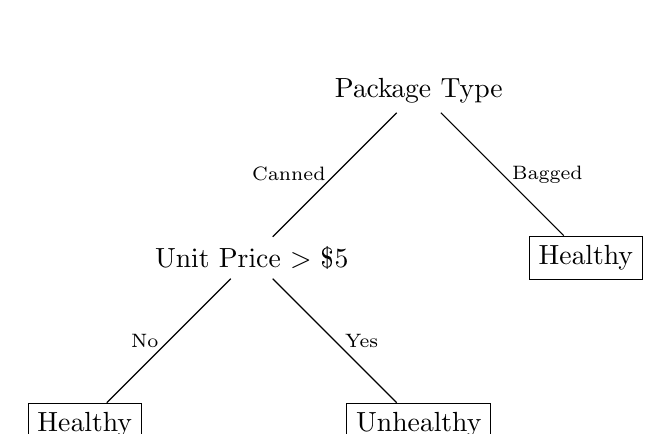
\begin{tikzpicture}
\node (a) at (0, 0) {Package Type};
\node (b) at (225: 3) {Unit Price $>$ \$5};
\node [draw, rectangle] (c) at (-45: 3) {Healthy};
\draw (a.225) -- (b.45);
\draw (a.-45) -- (c.135);
\node [left] at (225:1.5) {\scriptsize Canned};
\node [right] at (-45:1.5) {\scriptsize Bagged};
\begin{scope}[shift={(225:3)}]
\node [draw, rectangle] (d) at (225:3) {Healthy};
\node [draw, rectangle] (e) at (-45:3) {Unhealthy};
\node [left] at (225:1.5) {\scriptsize No};
\node [right] at (-45:1.5) {\scriptsize Yes};
\draw (b.225) -- (d.45);
\draw (b.-45) -- (e.135);
\end{scope}
\end{tikzpicture}
\end{figure}
\item No. For example in Figure \ref{perceptron vs tree} we clearly see that for this linearly separable data, the perceptron is much simpler than the tree, and both have zero training error.
\begin{figure}[h!]
\centering
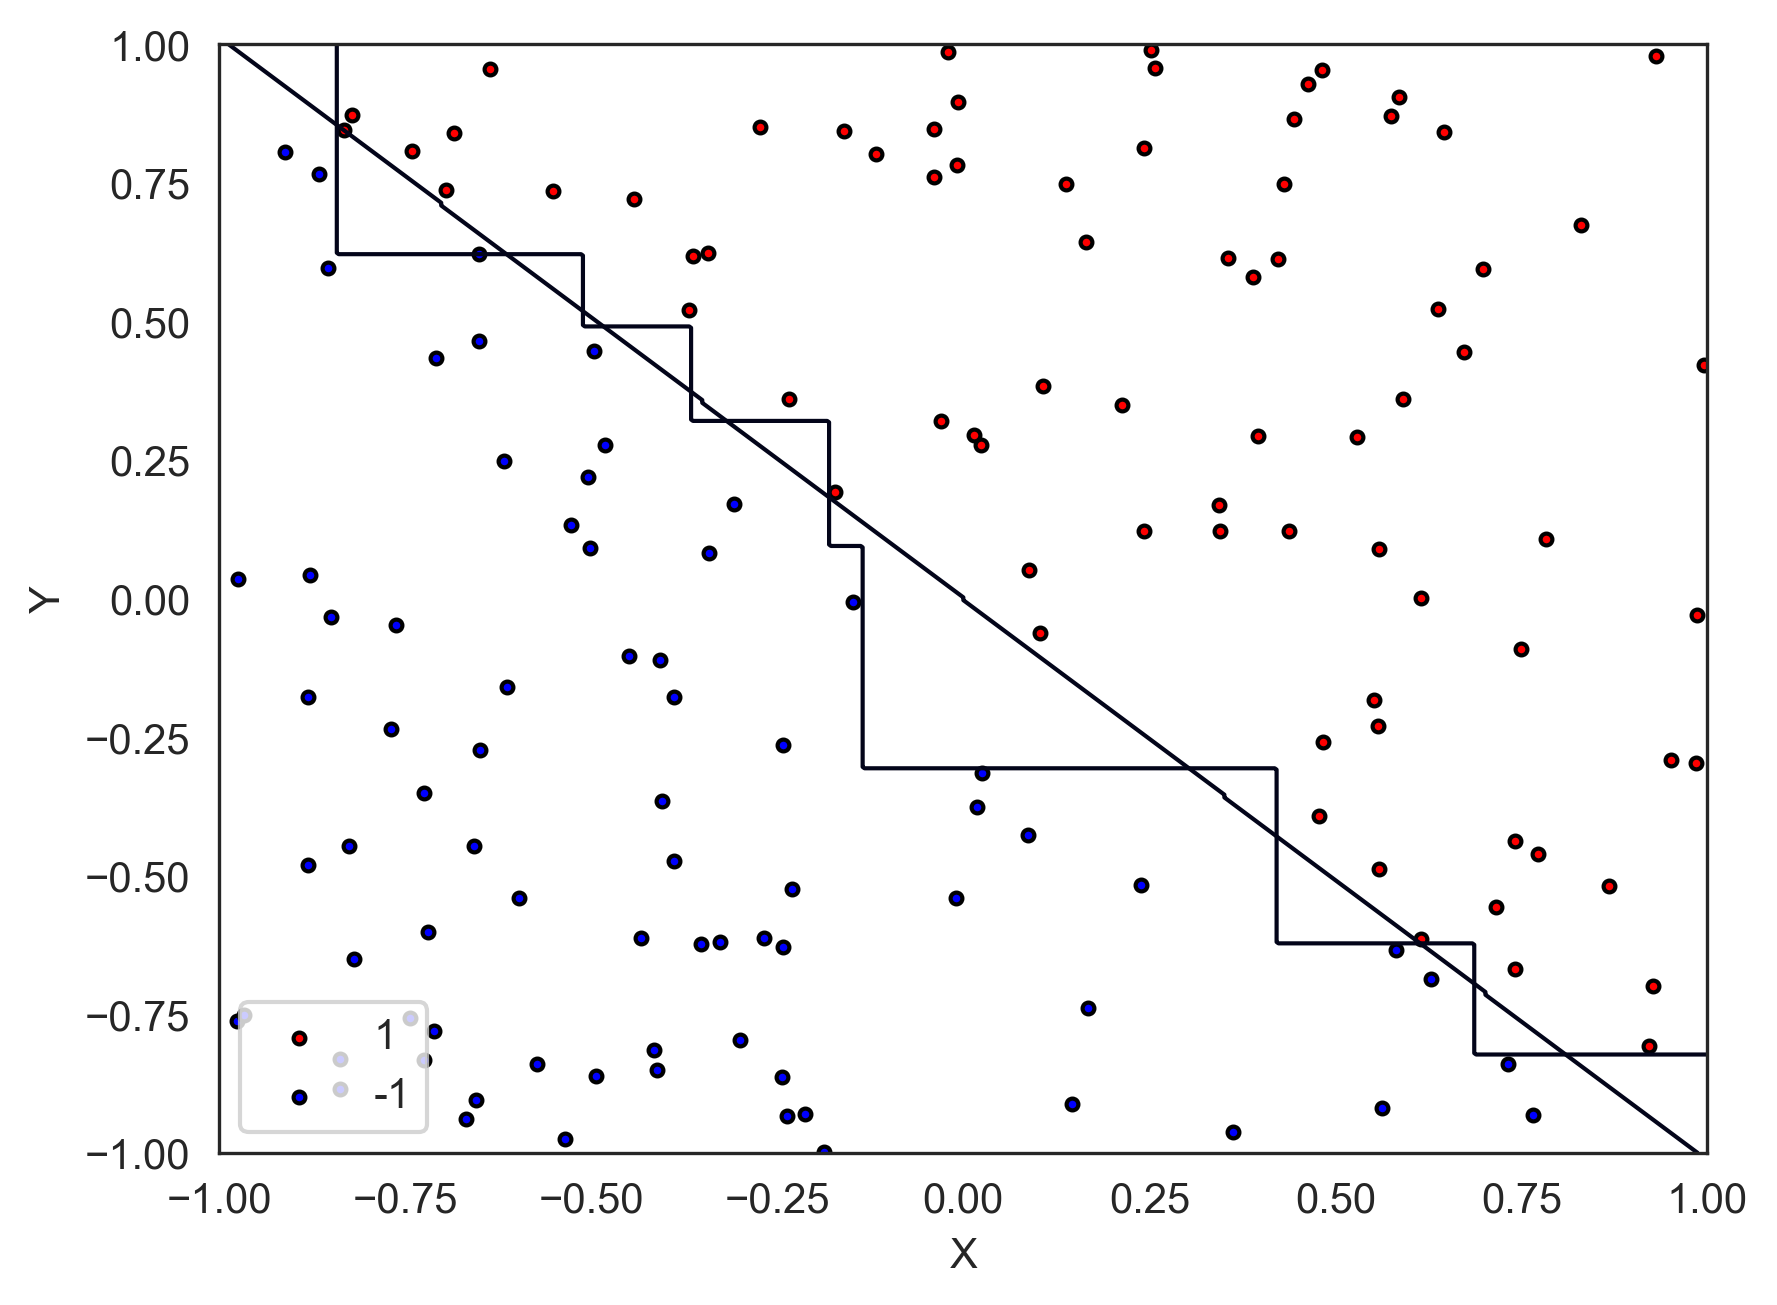
\includegraphics[scale=0.65]{Set3Figures/random_linear.png}
\caption{Training linearly separable data with perceptron versus tree classifier.} \label{perceptron vs tree}
\end{figure}
\item
\begin{enumerate}
\item The initial loss according to the gini index is ($p_S = 0.5$)
\[ L(S) = 4 \left( 1 - \frac{1}{4} - \frac{1}{4} \right) = 2 \]
A single split along the vertical axis $(x_2 = 0)$ yields
\[ L(S) = 1 + 1 = 2, \]
so there's no reduction in impurity. The same results in a split along $x_1 = 0$. So the classification error is 0.5.
\item The tree with no training error is shown below in Figure \ref{tree}.
\begin{figure}[h!]
\centering
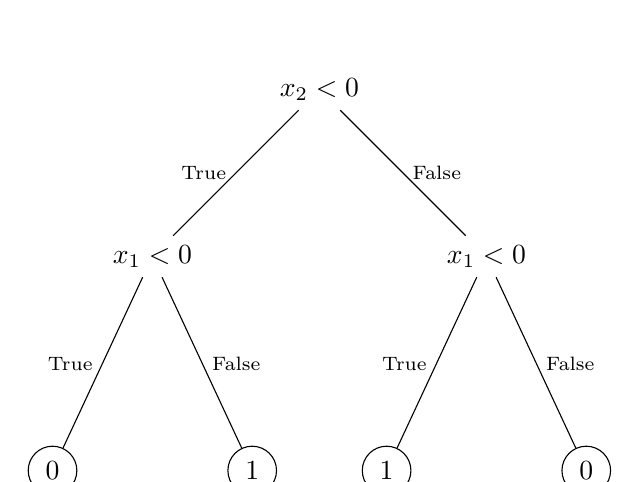
\begin{tikzpicture}
\node (a) at (0, 0) {$x_2 < 0$};
\node (b) at (225: 3) {$x_1 < 0$};
\node (c) at (-45: 3) {$x_1 < 0$};
\draw (a.225) -- (b.45);
\draw (a.-45) -- (c.135);
\node [left] at (225:1.5) {\scriptsize True};
\node [right] at (-45:1.5) {\scriptsize False};
\begin{scope}[shift={(225:3)}]
\node [draw, circle] (d) at (245: 3) {0};
\node [draw, circle] (e) at (-65: 3) {1};
\draw (b.245) -- (d.65);
\draw (b.-65) -- (e.115);
\node [left] at (245: 1.5) {\scriptsize True};
\node [right] at (-65: 1.5) {\scriptsize False};
\end{scope}
\begin{scope}[shift={(-45:3)}]
\node [draw, circle] (f) at (245: 3) {1};
\node [draw, circle] (g) at (-65: 3) {0};
\draw (c.245) -- (f.65);
\draw (c.-65) -- (g.115);
\node [left] at (245: 1.5) {\scriptsize True};
\node [right] at (-65 : 1.5) {\scriptsize False};
\end{scope}
\end{tikzpicture}
\caption{Tree for 4 data points in Problem C.} \label{tree}
\end{figure}
\item Yes, we could have the impurity measure
\[ L(S) = |S|^2 \left( 1 - p_S^2 - (1 - p_S)^2 \right). \]
This would create the tree shown in Figure \ref{tree}. The problem with this loss metric is that while it prioritizes too much on the size of the dataset size with the $|S|^2$ factor. As a result, a node prioritizes making the two children nodes have equal sizes over separating classes.
\item In the worst case scenario, each partition or leaf only contains one point in the training set. Therefore, we need at least 100 leaf nodes. Starting at the root node corresponding to depth level $\ell = 0$, the $n$th depth level has $2^\ell$ nodes. Note that $2^6 = 64$, so we need at least 7 levels, where the 7th level has $2 \times (100 - 64) = 72$ nodes (all of them leaf nodes). As a result, the 6th level has $36$ internal nodes. Summing from the root to the 5th level internal nodes yields
\[ \sum_{k = 0}^5 2^k = 63. \]
Therefore, the number of internal nodes in the worst case scenario of every leaf node containing one point gives $63 + 36 = 99$ internal nodes. Of course, most datapoints won't produce trees with 99 data points (the average value is about 36 nodes from averaging random datasets).
\end{enumerate}
\item For each continuous feature, we must consider $N - 1$ splits. Therefore, we must consider $D (N - 1)$ splits $\sim O(ND)$.
\end{enumerate}
\item
\begin{enumerate}[label=\Alph*.]
\item We see from Figure \ref{leaf} that from the $\Eout$ curve, the optimal minimum leaf size for this dataset is 12.
\begin{figure}[h!]
\centering
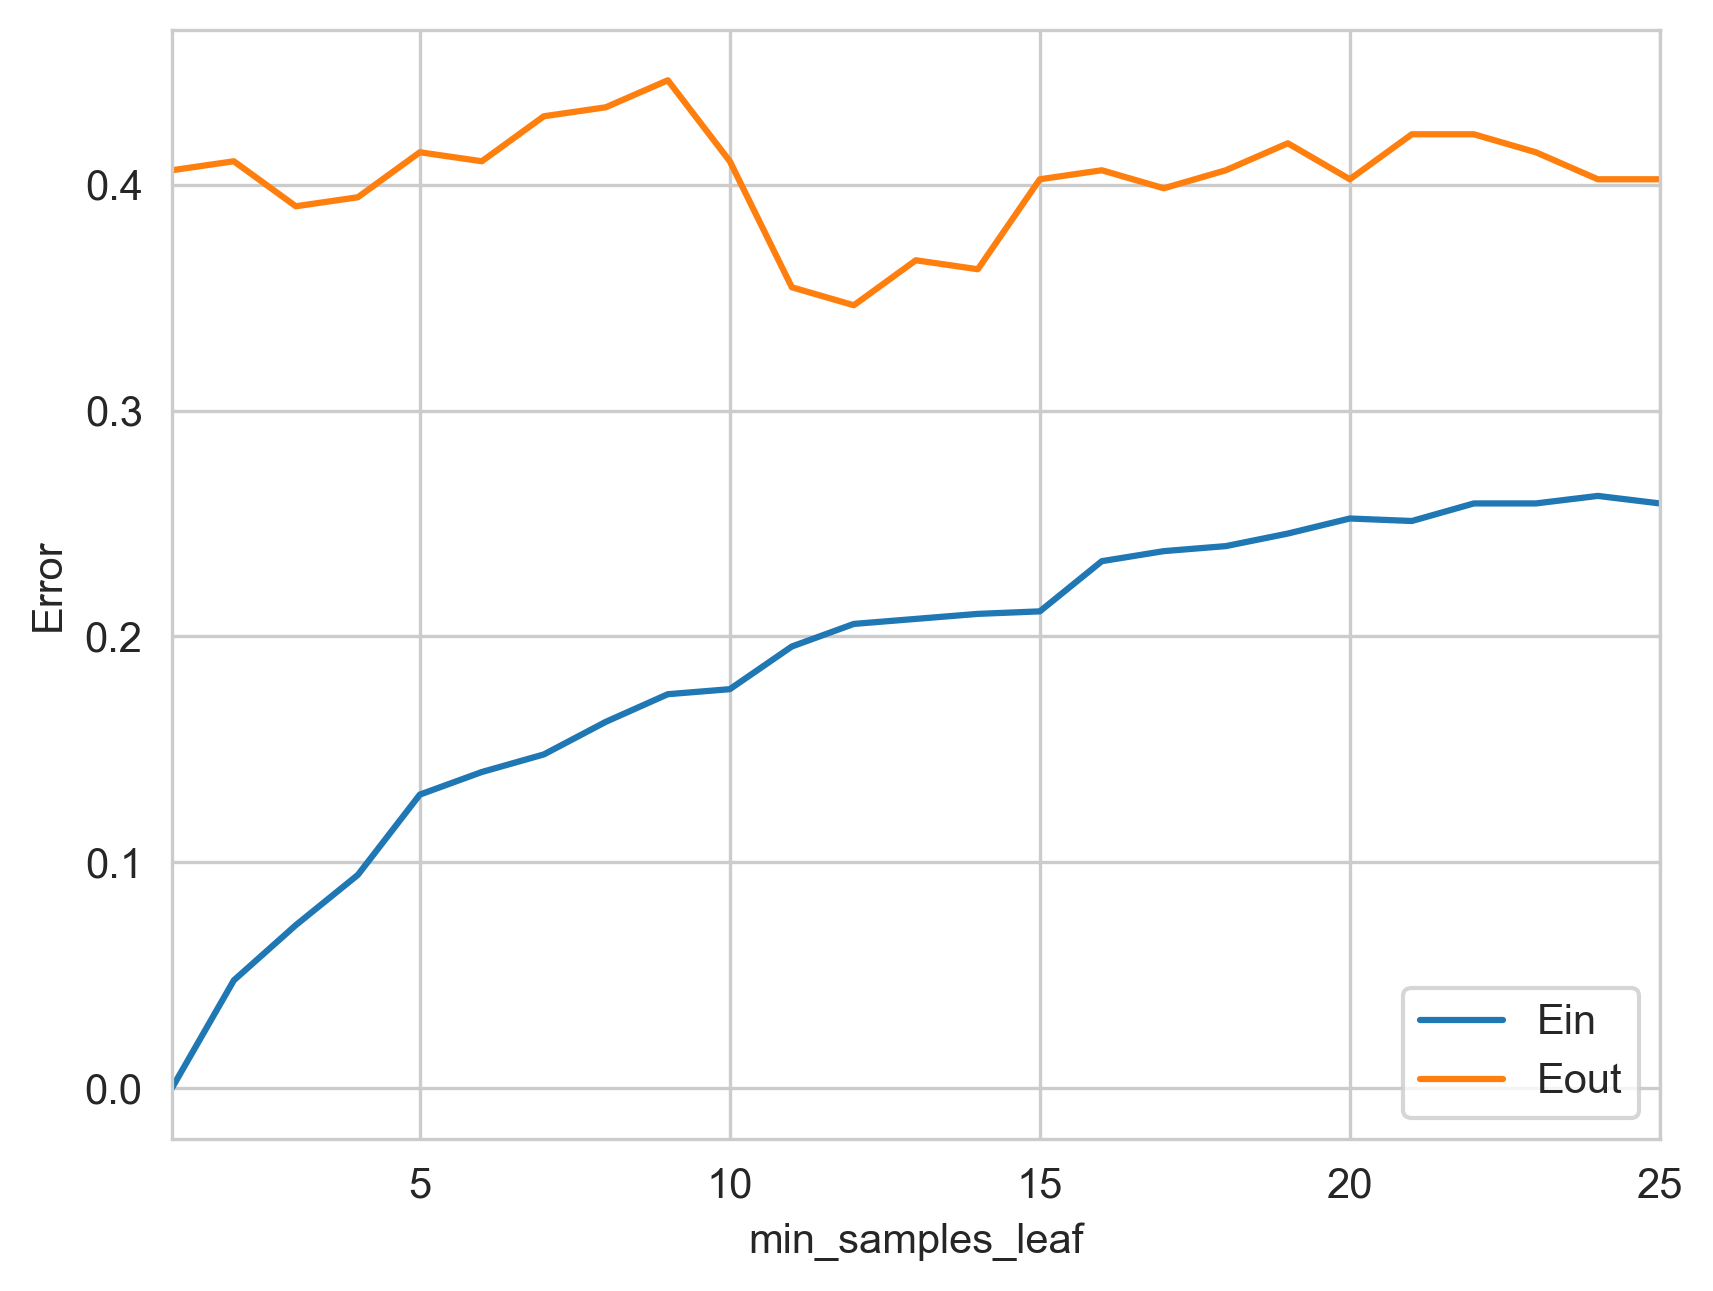
\includegraphics[scale = 0.5]{Set3Figures/minleafsize.png}
\caption{The optimal leaf size is 12.} \label{leaf}
\end{figure}
\item We see from Figure \ref{depth} that from the $\Eout$ curve, the optimal depth for the tree is 2.
\begin{figure}[h!]
\centering
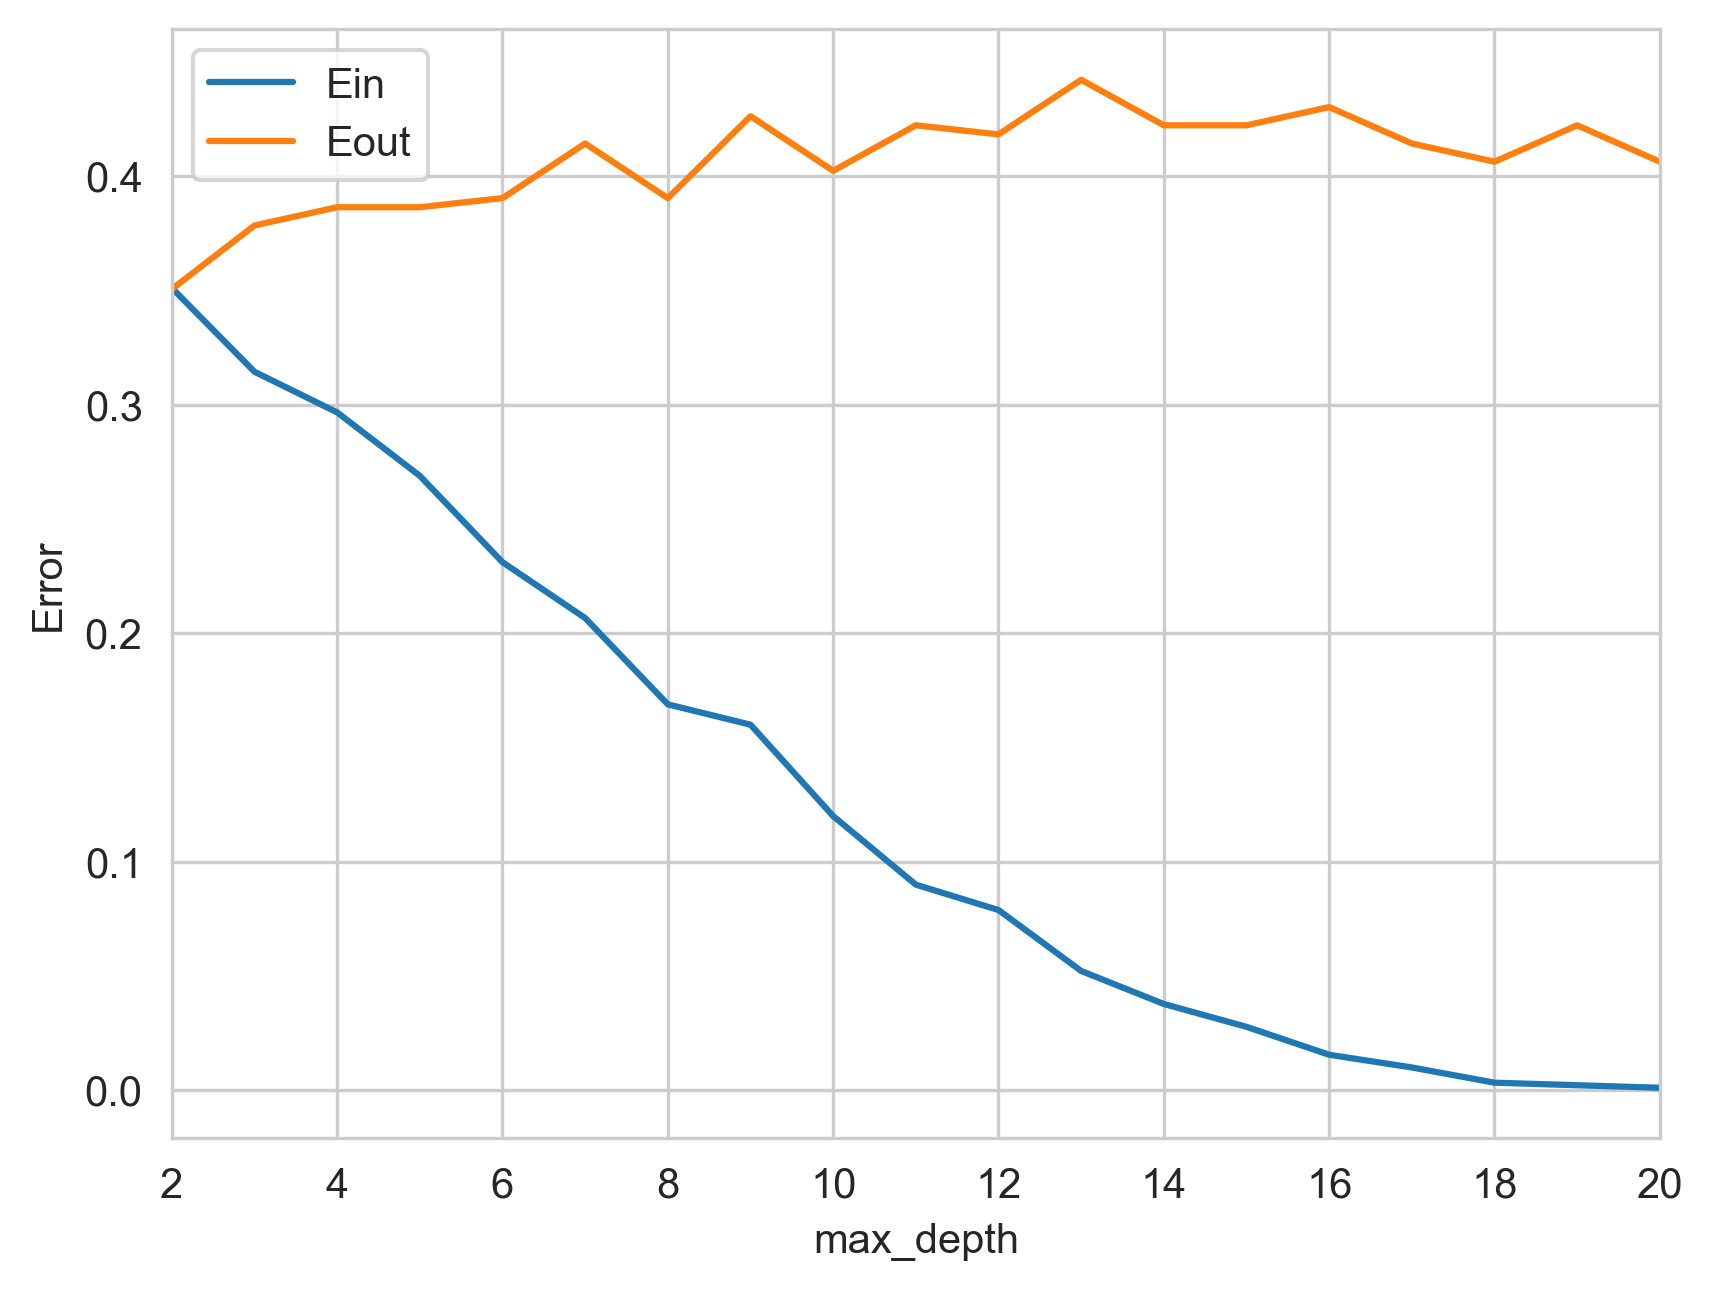
\includegraphics[scale=0.5]{Set3Figures/maxdepth.png}
\caption{The optimal depth is 2.} \label{depth}
\end{figure}
\item We see that neither stopping criterion has a profound impact on the accuracy of the model. We see some overfitting in the depth.
\item We see from Figure \ref{leafrf} that from the $\Eout$ curve, the optimal minimum leaf sisze for the tree is 3.
\begin{figure}[h!]
\centering
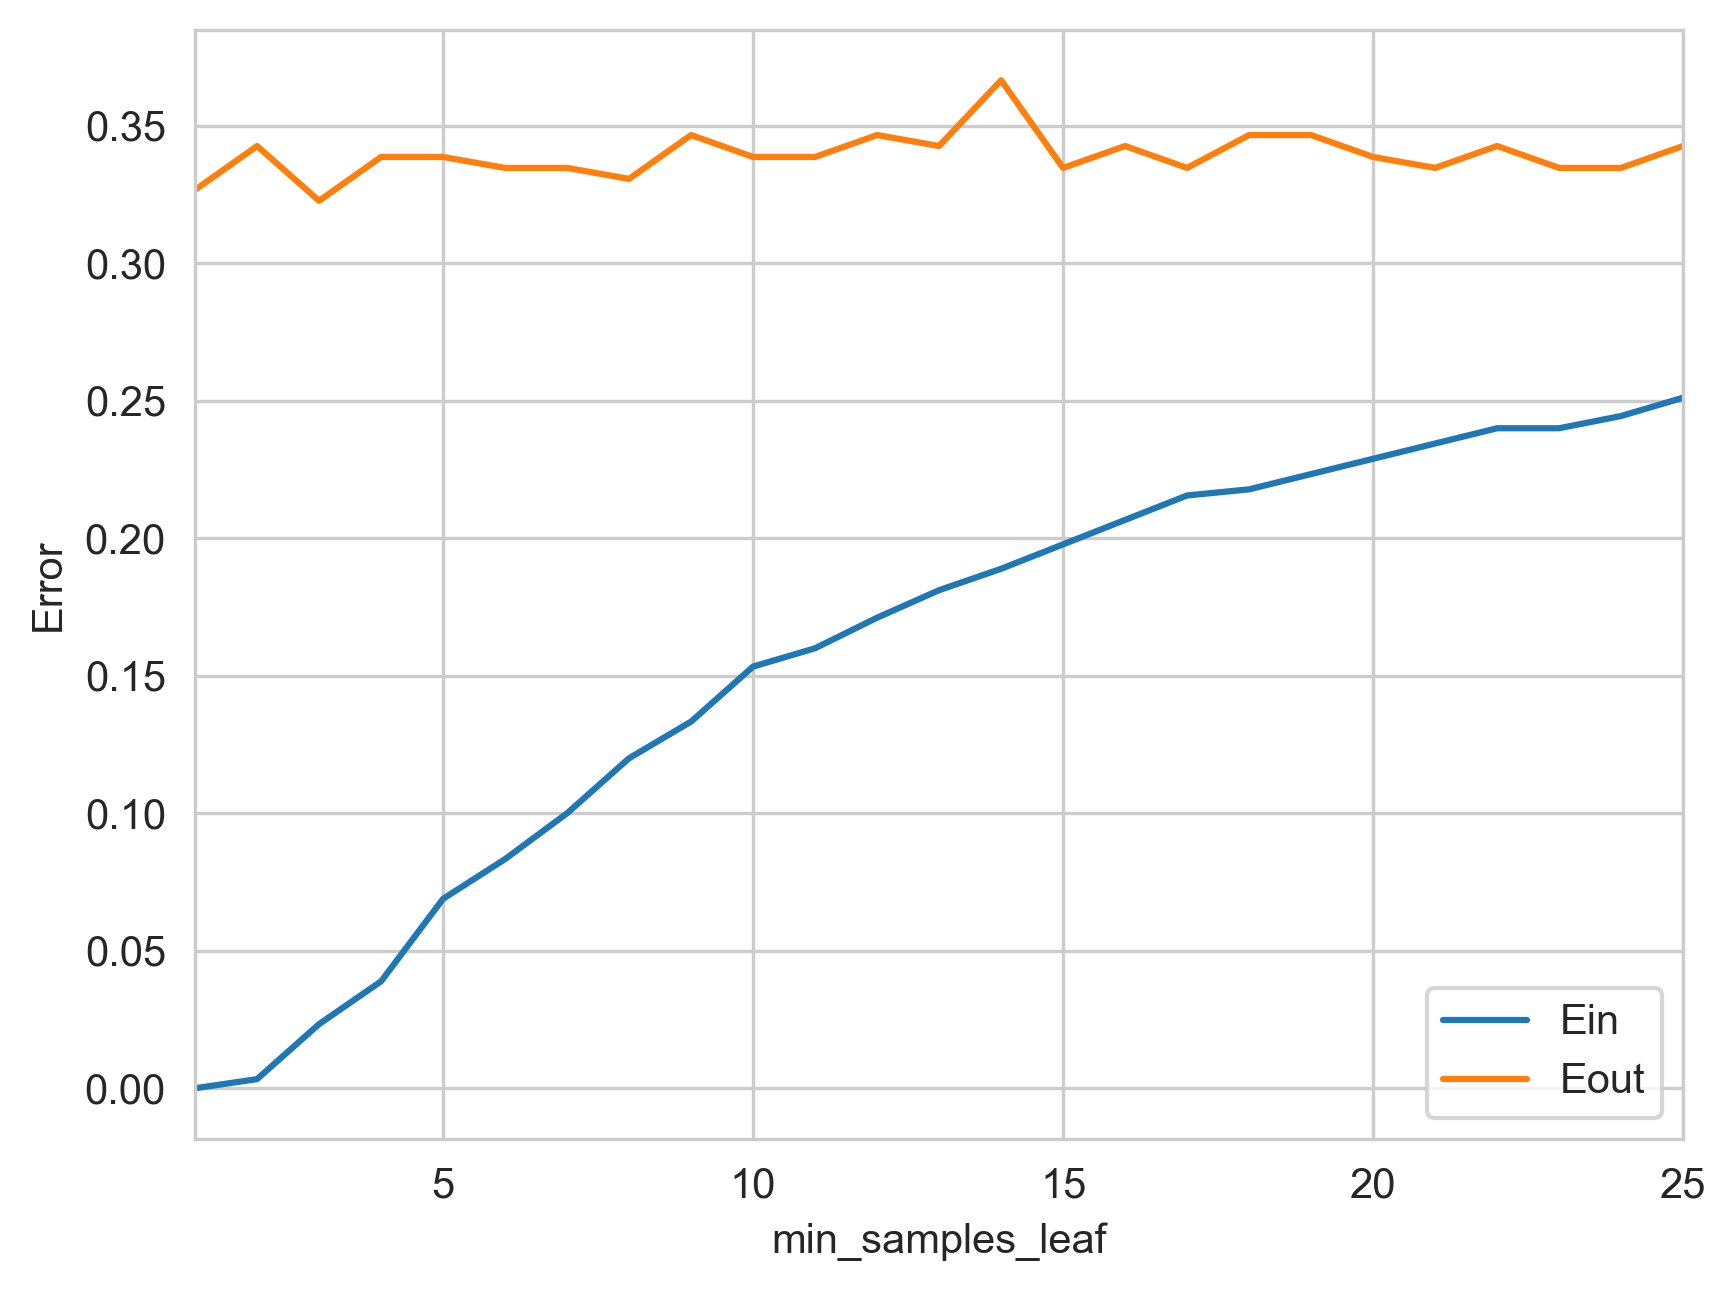
\includegraphics[scale=0.5]{Set3Figures/minleafsizerf.png}
\caption{The optimal leaf size is 3.} \label{leafrf}
\end{figure}
\item We see from Figure \ref{depthrf} that from the $\Eout$ curve, the optimal depth for the tree is 12.
\begin{figure}[h!]
\centering
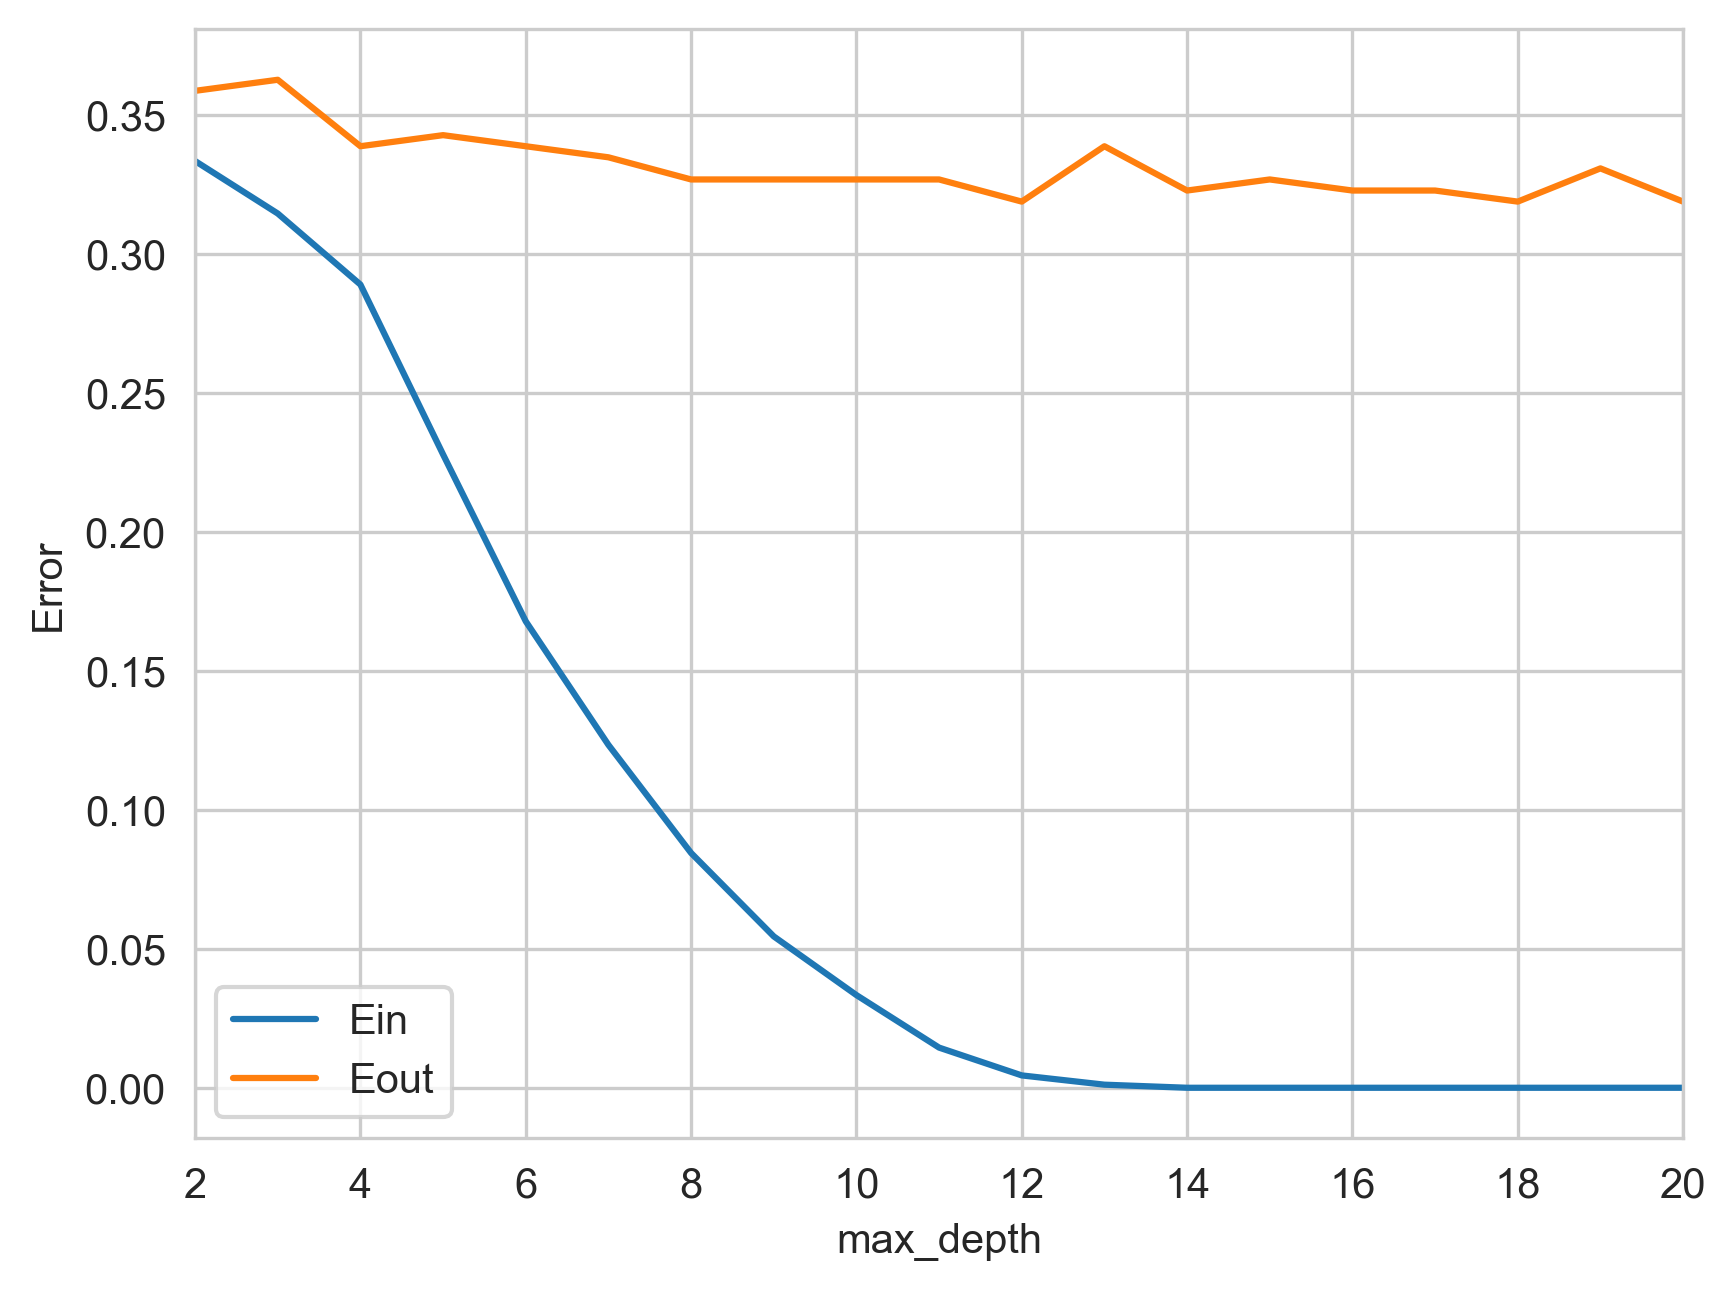
\includegraphics[scale=0.5]{Set3Figures/maxdepthrf.png}
\caption{The optimal depth is 12.} \label{depthrf}
\end{figure}
\item The early stopping on leaf size has little effect on the model accuracy. However, it does seem that depth has a stronger effect than leaf size.
\item The depth curve for the tree increases while it decreases for the random forest. The reason could be that the variance for the tree is greater than that for the random forest, so the $\Eout$ curve for this particular train-test split has this characterization. The random forest has a smaller variance, and so it produces an $\Eout$ curve more similar to what we would expect.
\end{enumerate}
\item
\begin{enumerate}[label=\Alph*.]
\item We look at the term
\[ E = \frac{1}{N} \sum_{i = 1}^N \exp \left(-y_i f(x_i) \right). \]
Now because $y_i$ and $f(x_i)$ have the same or opposite signs, it follows that if $y_i$ and $f(x_i)$ have the same size, then the term in the exponent is negative, so
\[ 0 < \exp \left( - y_i f(x_i) \leq 1 \right), \qquad y_i f(x_i) \geq 0 \]
and similarly if they have opposite signs
\[ 1 \leq \exp \left(- y_i f(x_i) \right), \qquad y_i f(x_i) \leq 0. \]
In either case, we see that
\[ \exp \left( -y_i f(x_i) \right) \geq \mathbbm{1} \left( H(x_i) \neq y_i \right), \]
so the desired result follows:
\[ \frac{1}{N} \sum_{i = 1}^N \exp \left( - y_i f(x_i) \right) \geq \frac{1}{N} \sum_{i = 1}^N \mathbbm{1} \left(H(x_i) \neq y_i \right). \]
\item We have
\[ D_{t + 1}(i) = \frac{1}{Z_t} D_t(i) \exp \left( -\alpha_t y_i h_t(x_i) \right). \]
We substitute recursively and note that $D_1(i) = 1 / N$, so we have
\[ D_{T + 1}(i) = \frac{1}{N} \prod_{t = 1}^T \frac{1}{Z_t} \exp \left( - \alpha_t y_i h_t(x_i) \right). \]
\item Just plug in $f(x_i)$ as the weighted sum of weak classifiers.
\begin{align*}
E &= \frac{1}{N} \sum_{i = 1}^N \exp \left(- y_i f(x_i) \right) \\
&= \frac{1}{N} \sum_{i = 1}^N \exp \left(- y_i \sum_{t = 1}^T \alpha_t h_t(x_i) \right).
\end{align*}
\item Expanding the result in C and using the result from B, we have
\begin{align*}
E &= \frac{1}{N} \sum_{i = 1}^N \exp \left( - \sum_{t = 1}^T \alpha_t y_i h_t(x_i) \right) \\
&= \frac{1}{N} \sum_{i = 1}^N \left[ \prod_{t = 1}^T \exp \left( - \alpha_t y_i h_t (x_i) \right) \right] \\
&= \frac{1}{N} \sum_{i = 1}^N \left[ D_{T + 1}(i) \prod_{t = 1}^T Z_t \right] \\
&= \prod_{t = 1}^T Z_t.
\end{align*}
In the last step, we used the fact that the $D_t$'s over $i$ must sum to $1$ and $Z_t$ is independent of $i$ and can be pulled out of the summation.
\item We have
\[ Z_t = \sum_{i = 1}^N D_t(i) \exp \left( - \alpha_t y_i h_t(x_i) \right). \]
We can rewrite the exponential factor as
\[ \exp \left( - \alpha_t y_i h_t(x_i) \right) = e^{-\alpha_t} + \left( e^{\alpha_t} - e^{-\alpha_t} \right) \mathbbm{1}(h_t(x_i) \neq y_i). \]
Therefore,
\begin{align*}
Z_t &= \sum_{i = 1}^N \left[ D_t(i) e^{-\alpha_t} + D_t(i) \left( e^{\alpha_t} - e^{-\alpha_t} \right) \mathbbm{1}(h_t(x_i) \neq y_i) \right] \\
&= e^{-\alpha_t} + \epsilon_t \left(e^{\alpha_t} - e^{-\alpha_t} \right) \\
&= \epsilon_t e^{\alpha_t} + (1 - \epsilon_t) e^{-\alpha_t}
\end{align*}
\item Differentiating $Z_t$ with respect to $\alpha_t$ and setting the result to zero yields
\begin{align*}
\epsilon_t e^{\alpha_t} + (\epsilon_t - 1) e^{- \alpha_t} &= 0 \\
\epsilon_t e^{2 \alpha_t} &= 1 - \epsilon_t \\
\alpha_t &= \frac{1}{2} \ln \left( \frac{1 - \epsilon_t}{\epsilon_t} \right).
\end{align*}
\end{enumerate}
\end{enumerate}

\end{document}